\documentclass[tikz,border=10pt,multi=tikzpicture]{standalone}
\usepackage{amsmath}
\usetikzlibrary{arrows.meta}

% Illustrative angles (any 0 < theta < phi < 90 degrees works)
\newcommand{\thetaDeg}{30}
\newcommand{\phiDeg}{50}

\colorlet{cosc}{blue!75!black}   % color for the cos(theta) vector (figures 2 and 4)
\colorlet{sinc}{red!75!black}    % color for the sin(theta) vector (figures 3 and 4)

\tikzset{
  axis/.style={-{Stealth[length=2.5mm]}, black!70},
  >={Stealth[length=2.5mm]},
}

\begin{document}

%% ------------------------------------------------------------------
%% Figure 1: rotating (1,0) and (0,1) by phi
%% ------------------------------------------------------------------
\begin{tikzpicture}[scale=3.2]
  \pgfmathsetmacro{\phiEnd}{90+\phiDeg}

  \draw[axis] (-1.3,0) -- (1.35,0) node[right] {$x$};
  \draw[axis] (0,-1.3) -- (0,1.35) node[above] {$y$};
  \draw[dashed, black!70] (0,0) circle (1);

  % terminal rays
  \draw[black!50] (0,0) -- (\phiDeg:1);
  \draw[black!50] (0,0) -- (\phiEnd:1);

  % rotation arcs
  \draw[->, very thick, cosc] (1,0) arc (0:\phiDeg:1);
  \draw[->, very thick, sinc] (0,1) arc (90:\phiEnd:1);

  % angle markers
  \draw[cosc] (0.28,0) arc (0:\phiDeg:0.28);
  \node[cosc] at ({\phiDeg/2}:0.42) {$\varphi$};
  \draw[sinc] (90:0.28) arc (90:\phiEnd:0.28);
  \node[sinc] at ({90+\phiDeg/2}:0.42) {$\varphi$};

  % points
  \fill (1,0) circle (0.9pt) node[below right] {$(1,0)$};
  \fill (0,1) circle (0.9pt) node[above right] {$(0,1)$};
  \fill[cosc] (\phiDeg:1) circle (0.9pt)
      node[above right] {$(\cos\varphi,\ \sin\varphi)$};
  \fill[sinc] (\phiEnd:1) circle (0.9pt)
      node[above left] {$(-\sin\varphi,\ \cos\varphi)$};
\end{tikzpicture}

%% ------------------------------------------------------------------
%% Figure 2: rotating (cos theta, 0) by phi
%% ------------------------------------------------------------------
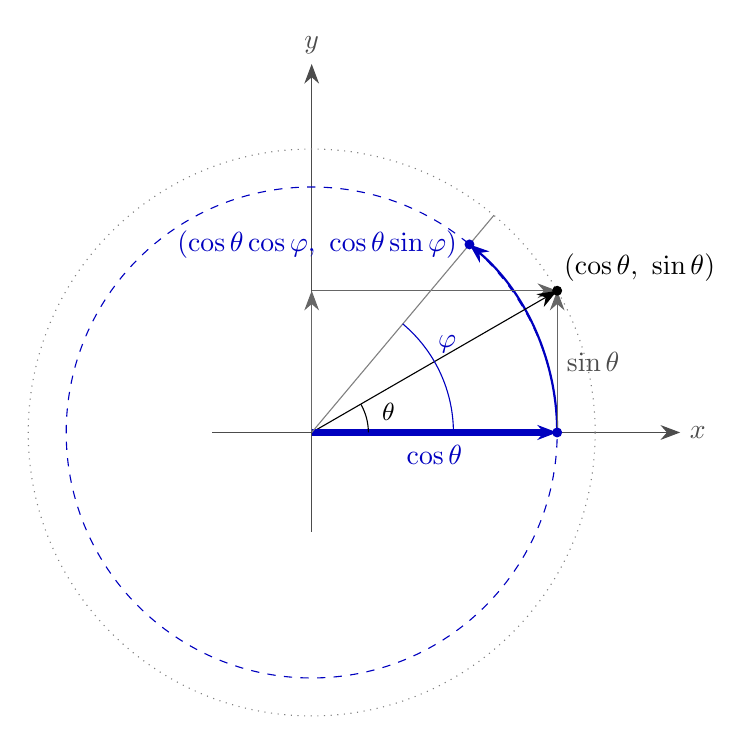
\begin{tikzpicture}[scale=3.6]
  \pgfmathsetmacro{\ct}{cos(\thetaDeg)}
  \pgfmathsetmacro{\st}{sin(\thetaDeg)}

  \draw[axis] (-0.35,0) -- (1.3,0) node[right] {$x$};
  \draw[axis] (0,-0.35) -- (0,1.3) node[above] {$y$};
  \draw[dotted, black!50] (0,0) circle (1);

  % circle of radius cos(theta) and the rotation of (cos theta, 0) by phi
  \draw[dashed, cosc] (0,0) circle (\ct);
  \draw[->, thick, cosc] (\ct,0) arc (0:\phiDeg:\ct);

  % vector addition, both ways, to reach (cos theta, sin theta)
  \draw[->, thin, black!60] (\ct,0) -- (\ct,\st);
  \draw[->, thin, black!60] (0,0) -- (0,\st);
  \draw[->, thin, black!60] (0,\st) -- (\ct,\st);
  \draw[->, black] (0,0) -- (\ct,\st);

  % emphasized horizontal component
  \draw[->, line width=2.2pt, cosc] (0,0) -- (\ct,0);

  % labels for the sum
  \fill (\ct,\st) circle (0.5pt)
      node[above right, xshift=-1pt] {$(\cos\theta,\ \sin\theta)$};
  \node[below, cosc] at ({\ct/2},-0.01) {$\cos\theta$};
  \node[right, black!70] at (\ct,{\st/2}) {$\sin\theta$};
  \draw[black] (0.2,0) arc (0:\thetaDeg:0.2);
  \node at ({\thetaDeg/2}:0.28) {\small$\theta$};

  % rotation by phi
  \draw[black!50] (0,0) -- (\phiDeg:1.0);
  \draw[cosc] (0.5,0) arc (0:\phiDeg:0.5);
  \node[cosc] at ({\phiDeg/2+8}:0.57) {$\varphi$};
  \fill[cosc] (\ct,0) circle (0.5pt);
  \fill[cosc] ({\ct*cos(\phiDeg)},{\ct*sin(\phiDeg)}) circle (0.5pt)
      node[left, xshift=-1pt, align=center]
      {$(\cos\theta\cos\varphi,\ \cos\theta\sin\varphi)$};
\end{tikzpicture}

%% ------------------------------------------------------------------
%% Figure 3: rotating (0, sin theta) by phi
%% ------------------------------------------------------------------
\begin{tikzpicture}[scale=3.6]
  \pgfmathsetmacro{\ct}{cos(\thetaDeg)}
  \pgfmathsetmacro{\st}{sin(\thetaDeg)}
  \pgfmathsetmacro{\phiEnd}{90+\phiDeg}

  \draw[axis] (-1.1,0) -- (1.3,0) node[right] {$x$};
  \draw[axis] (0,-0.35) -- (0,1.3) node[above] {$y$};
  \draw[dotted, black!50] (0,0) circle (1);

  % circle of radius sin(theta) and the rotation of (0, sin theta) by phi
  \draw[dashed, sinc] (0,0) circle (\st);
  \draw[->, thick, sinc] (0,\st) arc (90:\phiEnd:\st);

  % vector addition, both ways, to reach (cos theta, sin theta)
  \draw[->, thin, sinc] (\ct,0) -- (\ct,\st);
  \draw[->, thin, black!60] (0,0) -- (\ct,0);
  \draw[->, thin, black!60] (0,\st) -- (\ct,\st);
  \draw[->, black] (0,0) -- (\ct,\st);

  % emphasized vertical component
  \draw[->, line width=2.2pt, sinc] (0,0) -- (0,\st);

  \fill (\ct,\st) circle (0.5pt)
      node[above right, xshift=-1pt] {$(\cos\theta,\ \sin\theta)$};
  \node[below, black!70] at ({\ct/2},-0.02) {$\cos\theta$};
  \node[right, sinc] at (\ct,{\st/2}) {$\sin\theta$};
  \draw[black] (0.2,0) arc (0:\thetaDeg:0.2);
  \node at ({\thetaDeg/2}:0.28) {\small$\theta$};

  % rotation by phi (angle measured from the y axis)
  \draw[black!50] (0,0) -- (\phiEnd:0.85);
  \draw[sinc] (90:0.3) arc (90:\phiEnd:0.3);
  \node[sinc] at ({90+\phiDeg/2}:0.40) {\small$\varphi$};
  \fill[sinc] (0,\st) circle (0.5pt);
  \fill[sinc] ({-\st*sin(\phiDeg)},{\st*cos(\phiDeg)}) circle (0.5pt)
      node[left, xshift=-1pt, align=center]
      {$(-\sin\theta\sin\varphi,\ \sin\theta\cos\varphi)$};
\end{tikzpicture}

%% ------------------------------------------------------------------
%% Figure 4: sequential rotations: first by theta, then by phi
%% ------------------------------------------------------------------
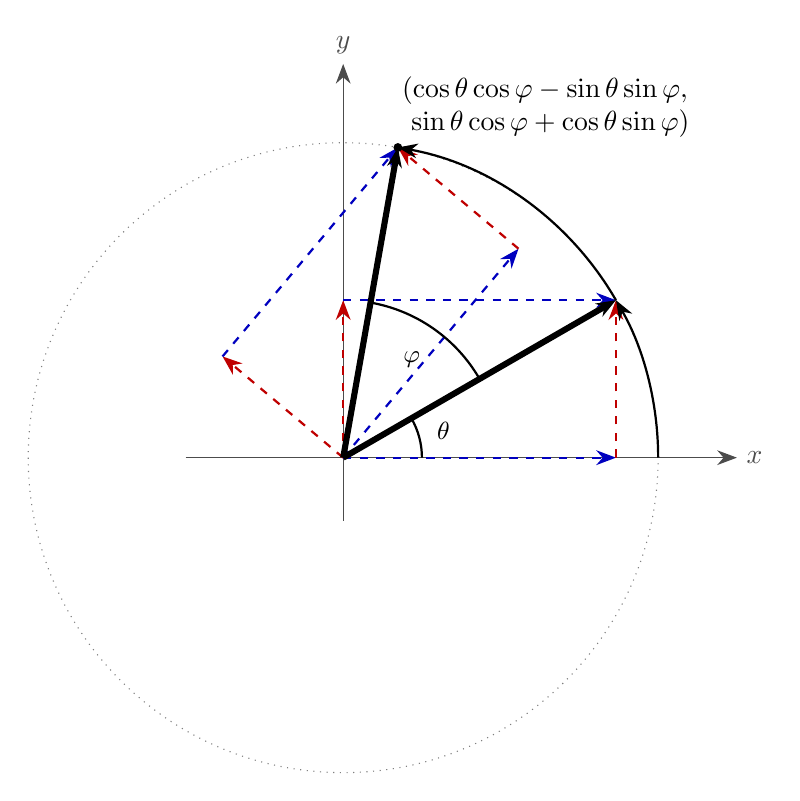
\begin{tikzpicture}[scale=4]
  \pgfmathsetmacro{\ct}{cos(\thetaDeg)}
  \pgfmathsetmacro{\st}{sin(\thetaDeg)}
  \pgfmathsetmacro{\Ax}{cos(\thetaDeg)*cos(\phiDeg)}
  \pgfmathsetmacro{\Ay}{cos(\thetaDeg)*sin(\phiDeg)}
  \pgfmathsetmacro{\Bx}{-sin(\thetaDeg)*sin(\phiDeg)}
  \pgfmathsetmacro{\By}{sin(\thetaDeg)*cos(\phiDeg)}
  \pgfmathsetmacro{\Sx}{\Ax+\Bx}
  \pgfmathsetmacro{\Sy}{\Ay+\By}
  \pgfmathsetmacro{\tp}{\thetaDeg+\phiDeg}

  \draw[axis] (-0.5,0) -- (1.25,0) node[right] {$x$};
  \draw[axis] (0,-0.2) -- (0,1.25) node[above] {$y$};
  \draw[dotted, black!50] (0,0) circle (1);

  % first rotation (by theta): components of (cos theta, sin theta), dashed
  \draw[->, dashed, thick, cosc] (0,0) -- (\ct,0);
  \draw[->, dashed, thick, sinc] (\ct,0) -- (\ct,\st);
  \draw[->, dashed, thick, sinc] (0,0) -- (0,\st);
  \draw[->, dashed, thick, cosc] (0,\st) -- (\ct,\st);

  % second rotation (by phi): rotated components and their parallel copies, dashed
  \draw[->, dashed, thick, cosc] (0,0) -- (\Ax,\Ay);
  \draw[->, dashed, thick, sinc] (0,0) -- (\Bx,\By);
  \draw[->, dashed, thick, sinc] (\Ax,\Ay) -- (\Sx,\Sy);
  \draw[->, dashed, thick, cosc] (\Bx,\By) -- (\Sx,\Sy);

  % rotation arc by theta from (1,0) to (cos theta, sin theta)
  \draw[->, thick, black] (1,0) arc (0:\thetaDeg:1);

  % rotation arc by phi from (cos theta, sin theta) to the final point
  \draw[->, thick, black] (\thetaDeg:1) arc (\thetaDeg:\tp:1);

  % bold black vector to (cos theta, sin theta)
  \draw[->, line width=2.2pt, black] (0,0) -- (\ct,\st);

  % bold black final vector
  \draw[->, line width=2.2pt, black] (0,0) -- (\Sx,\Sy);

  % angles: theta from the x axis, phi from the first rotated vector
  \draw[thick, black] (0.25,0) arc (0:\thetaDeg:0.25);
  \node at ({\thetaDeg/2}:0.33) {\small$\theta$};
  \draw[thick, black] (\thetaDeg:0.5) arc (\thetaDeg:\tp:0.5);
  \node at ({\thetaDeg+\phiDeg/2}:0.38) {\small$\varphi$};

  % only the final point is labeled
  \fill (\Sx,\Sy) circle (0.4pt)
      node[above right, xshift=-2pt, align=left]
      {$(\cos\theta\cos\varphi-\sin\theta\sin\varphi,$\\
        $\ \sin\theta\cos\varphi+\cos\theta\sin\varphi)$};
\end{tikzpicture}

\end{document}
